\documentclass{article}
\usepackage[utf8]{inputenc}
\usepackage[T2A]{fontenc}
\usepackage[russian]{babel}
\usepackage{secdot}
\usepackage{hyperref}
\usepackage[top=2cm,right=2cm,bottom=2cm,left=2cm]{geometry}

\title{Учим процессор расходовать ресурсы}
\author{Альберт Нагапетян, Семен Пьянков}
\date{}
\bibliographystyle{unsrt}

\usepackage{graphicx}
\graphicspath{{/Users/admin/Desktop/}}
\graphicspath{{/}}
\DeclareGraphicsExtensions{.pdf,.png,.jpg}

\begin{document}
\maketitle

\section{Постановка задачи}

Задача минимизировать суммарную энергию, потребляемую процессором, и найти распределение ресурсов по процессам и скоростей по времени. 
Энергия в каждый момент времени вычисляется по закону $ \alpha + \beta x_i + \gamma x_i^2$, $x_i$ - скорость процессора в момент времени i. Тогда нужно минимизировать сумму энергий, затраченных в каждый момент времени: $\min \sum \limits_{i=0}^{T-1} \alpha + \beta x_i + \gamma x_i^2$\\

На скорость условиями задачи накладываются ограничения: $S_{min} \le x_i \le S_{max}$, $S_{min}, S_{max}$ - минимальная и максимальная скорости, даны в условии. Кроме того, ограничения касаются и приращения скорости, то есть две подрядыдущих скорости отличаются не более, чем на определенную условием константу $R$: $|x_i-x_{i-1}| \le R ~~ \forall i = 1 \dots T-1$, где T - суммарное время работы процессора. \\

Скорость в каждый момент времени зависит от того, сколько ресурсов нужно затратить на процессы в каждый момент времени:
$x_i = \sum \limits_{j=0}^{n-1} X_{ij}$, $n$ - число задач, $X_{ij}$ - объем ресурсов, затраченный в i-ый момент времени j-ым процессом.\\

Кроме того, есть ограничение на суммарную работу, которую должен выполнить процессор: суммарный объём вычислений для каждой работы был не меньше требуемого для её выполнения\\
$\sum \limits_{i=0}^{T-1} X_{ij} \ge W_j$, где $W_j$ - работа, которую надо затратить для j-го процесса\\

%Тогда нужно вычислить до постановки задачи: \\
%$x_i = \sum\limits_j X_{ij}$\\
%$y_j = \sum\limits_i X_{ij}$\\
%$x^* = (x_1, \dots, x_{15})$\\
%$x_* = (x_0, \dots, x_{14})$\\

Получаем задачу:\\
$\min \alpha T + \mathbf{\beta^{\top}x} + \gamma \mathbf{x^{\top}x}$, где $x_i = \sum \limits_{j=0}^{n-1} X_{ij}$\\
s.t. $\mathbf{x} \succeq \mathbf{S_{min}} $\\
$\mathbf{x} \preceq \mathbf{S_{max}}$\\
$|x_{i} - x_{i-1}| \le R$\\
%$\mathbf{x_*} - \mathbf{x^*} \preceq \mathbf{R}$\\
$\mathbf{y} \succeq \mathbf{W}$, где $y_j = \sum\limits_i X_{ij}$\\


\section{Анализ задачи и описание алгоритмов её решения}

Недостатки постановки - не реализовано в матричной форме. Для краткости записи (да и простоты вычисления) было бы удобнее реализовать в виде матриц и векторов, но не все ограничения позволяют это сделать. Возможно, введя дополнительные переменные, можно было бы реализовать, но между экономией времени работы человека и машины мы решили сделать выбор в свою пользу.\\

Достоинства постановки - составлена задача квадратичного программирования с ограничениями типа равенства и неравенства. Эта задача выпуклая, а значил ее можно решать разными методами, в том числе: метод внутренней точки (в нашем случае использовался ECOS $\cite{Domahidi2013ecos}$), ADMM $\cite{Boyd2011}$ (в нашем случае использовался SCS). В общем случае, эти solverы решают выпуклые конические задачи, нашу задачу можно свести к задаче SOCP (second order cone problem), это делает cvxpy (функция \text{get\_problem\_data}). Плюсы этих методов в универсальности и отсутствии необходимости подключать какие-либо дополнительные библиотеки. \\


\section{Результаты экспериментов}

В результате вычислений методами ECOS и SCS мы получили распределение ресурсов по процессам:

\begin{figure}[h]
\begin{center}
\begin{minipage}[h]{8cm}
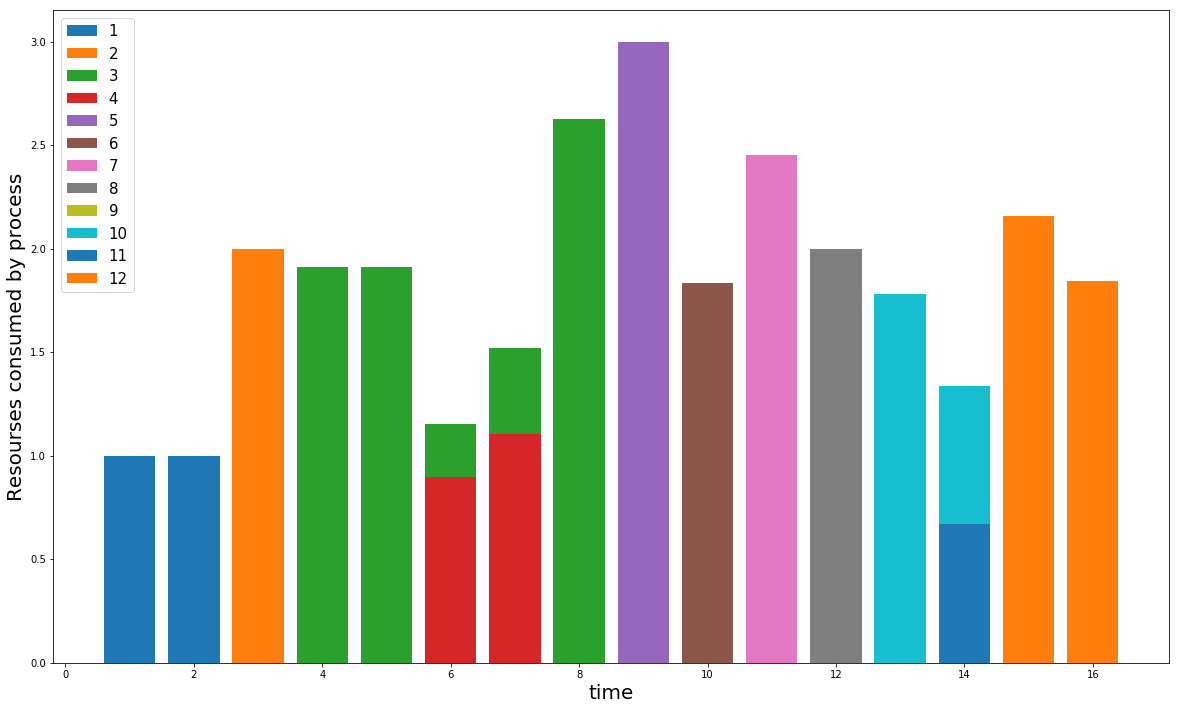
\includegraphics[width=8cm]{ECOS_2.png}
\caption{ECOS} %% подпись к рисунку
\label{ris:experimoriginal} %% метка рисунка для ссылки на него
\end{minipage}
\hfill 
\begin{minipage}[h]{8cm}
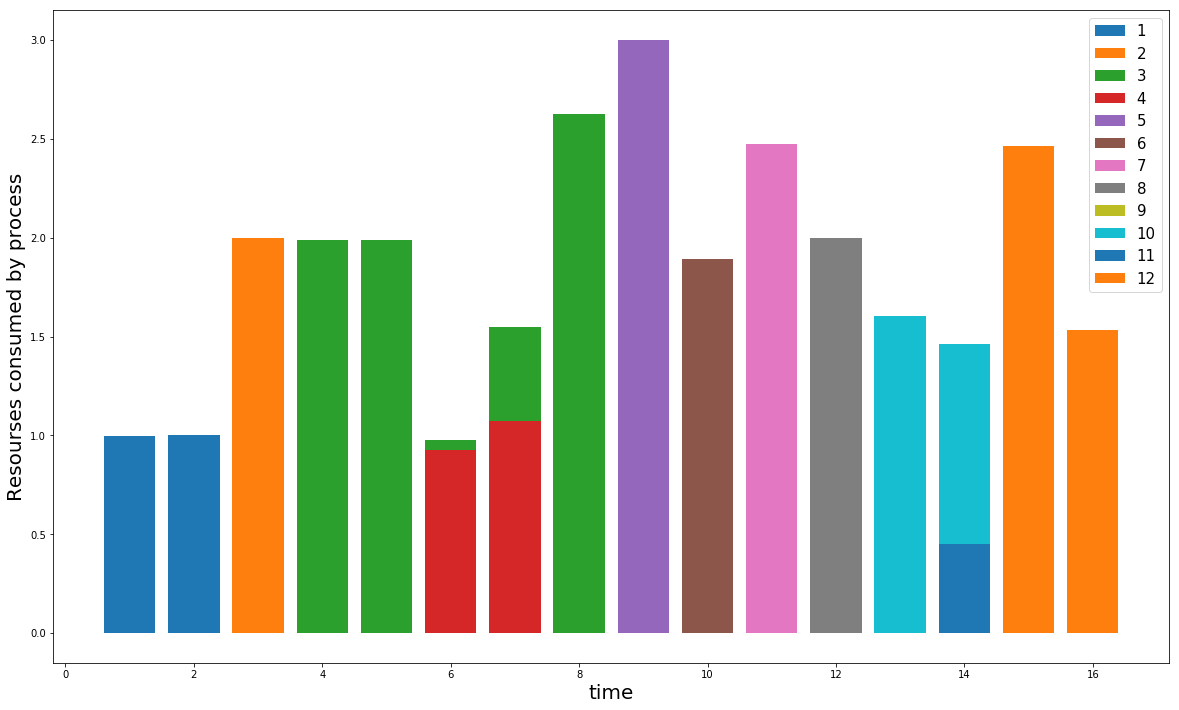
\includegraphics[width=8cm]{SCS_2.png}
\caption{SCS}
\label{ris:experimcoded}
\end{minipage}
\end{center}
\end{figure}

И значение скорости процессора во времени:\\

\begin{figure}[h]
\begin{center}
\begin{minipage}[h]{8cm}
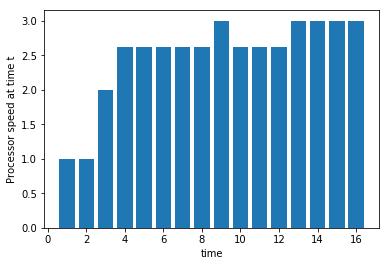
\includegraphics[width=8cm]{ECOS_3.png}
\caption{ECOS} %% подпись к рисунку
\label{ris:experimoriginal} %% метка рисунка для ссылки на него
\end{minipage}
\hfill 
\begin{minipage}[h]{8cm}
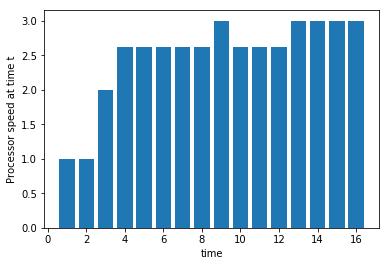
\includegraphics[width=8cm]{SCS_3.png}
\caption{SCS}
\label{ris:experimcoded}
\end{minipage}
\end{center}
\end{figure}

Также была оценена зависимость точности вычисления от числа итераций:\\

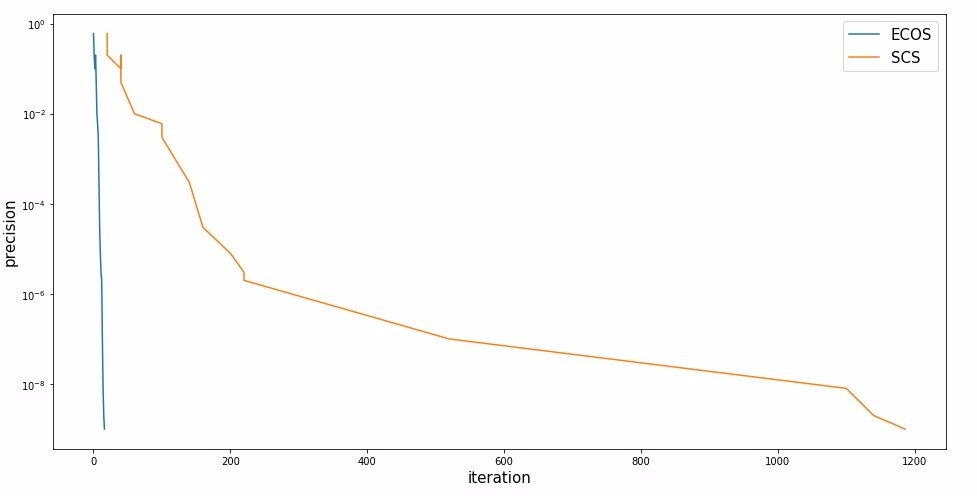
\includegraphics[width=12cm]{cmp.jpg}

И время исполнения итерации у ECOS: 

110 ms $\pm$ 572 $\mu$s per loop (mean $\pm$ std. dev. of 7 runs, 10 loops each)

И у SCS:

129 ms $\pm$ 750 $\mu$s per loop (mean $\pm$ std. dev. of 7 runs, 10 loops each)

Получили, что ECOS нужно сделать гораздо меньше итераций, чем SCS для достижения опеределенной точности, эти итерации работают примерно одинаковое (по порядку) количество времени, то есть по времени выгоднее пользоваться ECOS (метод внутренней точки).

В дополнении, мы также получили оценки зазора двойственности: 9e-07 для ECOS и 2.4e-12.

Однако, после некоторых раздумий, было принято за аксиому, что нагрузка (равно как и скорость) процессора должна быть целочисленная. Тогда была найдена модификация ECOS - ECOS\_BB:


\begin{figure}[h]
\begin{center}
\begin{minipage}[h]{8cm}
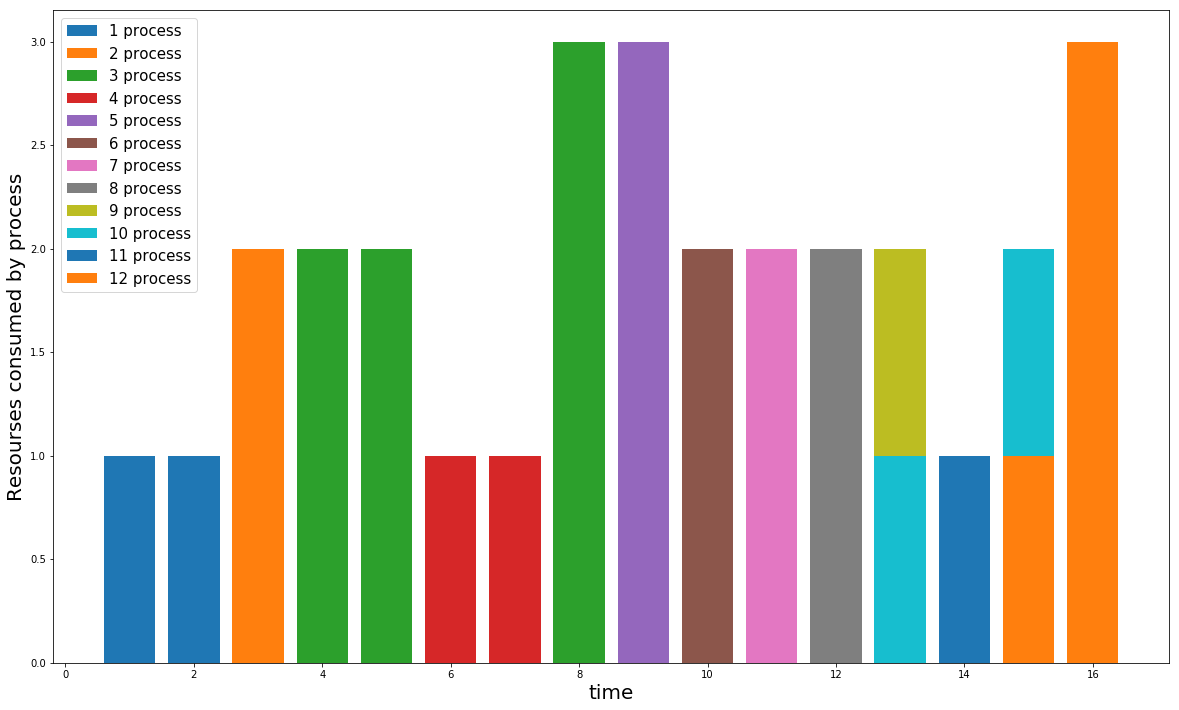
\includegraphics[width=8cm]{ECOSBB_2.png}
\caption{Распределение нагрузки} %% подпись к рисунку
\label{ris:experimoriginal} %% метка рисунка для ссылки на него
\end{minipage}
\hfill 
\begin{minipage}[h]{8cm}
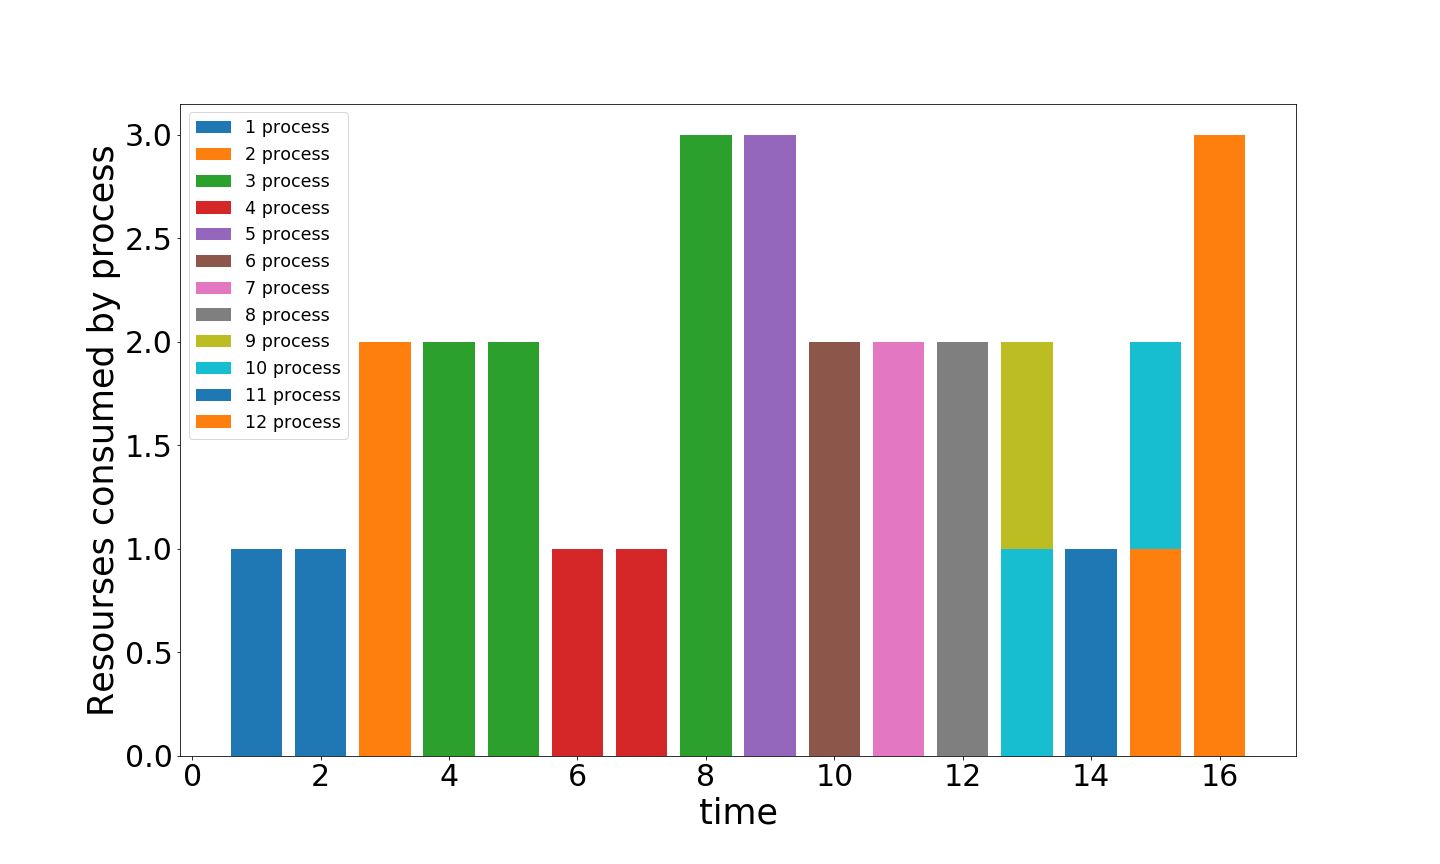
\includegraphics[width=8cm]{ECOSBB_3.png}
\caption{Скорость}
\label{ris:experimcoded}
\end{minipage}
\end{center}
\end{figure}


\section{Обсуждение}

Мы решили задачу, нашли распределения энергии и скорости процессора в каждый момент времени (в том числе и для целочисленного случая - более приближенного к реальности).

При решении возникла проблема с составлением задачи математического программирования. Чтобы упростить выражение, хотелось получить векторно-матричную форму записи. Но это не будет иметь особого смысла ($\succeq$ релаизуется все равно поэлементно, да и не очень понятно, как оформить ограничение $|x_i-x_{i-1}| \le R$ без введения дополнительных переменных). \\

Еще одна трудность - осознание целочисленности задачи. Из-за этого пришлось применять ECOS\_BB, который, конечно, дал решение, отличающееся от непрерывного случая. Скорее всего, при достаточно больших затратах, непрерывный случай будет точнее отображать реальные условия.\\

При первом прочтении условия показалось, что задача достаточно узкая, поскольку нужно знать точное расписание занятости процессора (то есть нужно знать, какие требуется запустить процессы в какое время и на какое время). Но как высяснилось, бывают и такие системы. К тому же, если не вдаваться в подробности, то планировщик операционной системы примерно так и составляет расписание (конечно задача усложняется тем, что мы не знаем, какие к нам придут задачи в будущем, но те задачи, которые известны, распределяются с минимальным потреблением ресурсов). Вообще это сильно упрощенная задача, но можно попытаться ее обобщить на многопоточную архитектуру, учесть ограничение на число процессов и попробовать реализовать решение задачи для реального планировщика (хотя в действительности проще пользоваться готовыми алгоритмами планирования, например из невытесняющих это FIFO, из вытесняющих - циклическая).\\

Кроме того, в многопоточных системах при использовании пула потоков возникает необходимость в статическом планировании. Потоки для фрагментов задания будут определяться заранее, наше решение поможет оптимизировать это распределение.\\

Еще одно применение - распределение задач в проекте внутри команды. Только необходимо ограничить число одновременно-запущенных процессов числом членов команды (или какой-то величиной, зависящей от этого числа).\\


\section{}\bibliography{CPUlibNEW}

\section{Роли}

\subsection{Формализация задачи (составление задачи математического программирования)} --- Семен Пьянков, Альберт Нагапетян
\subsection{Реализация на python:}
    \subsubsection{Поиск алгоритмов, которые позволяют решить эту задачу} --- Альберт Нагапетян, Семен Пьянков
    \subsubsection{Написание кода, решающего задачу с использованием этих алгоритмов} --- Альберт Нагапетян
    \subsubsection{Отладка} --- Альберт Нагапетян %:) как будто мы ей занимаемся 
\subsection{Обоснование решения} --- Семен Пьянков, Альберт Нагапетян
\subsection{Оформление отчета} --- Семен Пьянков
\subsection{Создание корректно оформленного репозитория на github} --- Семен Пьянков\\

На самом деле разделение очень условное, поскольку вносились изменения разного плана всеми участниками во все части проекта.\\



\end{document}
